\documentclass[10pt,english]{beamer}
\usepackage{lmodern}
\usepackage[T1]{fontenc}
\usepackage[utf8]{inputenc}
\setcounter{tocdepth}{1}
\usepackage{amsbsy}
\usepackage{amstext}
\usepackage{amssymb}
\usepackage[authoryear]{natbib}

\makeatletter
%%%%%%%%%%%%%%%%%%%%%%%%%%%%%% Textclass specific LaTeX commands.
% this default might be overridden by plain title style
\newcommand\makebeamertitle{\frame{\maketitle}}%
% (ERT) argument for the TOC
\AtBeginDocument{%
  \let\origtableofcontents=\tableofcontents
  \def\tableofcontents{\@ifnextchar[{\origtableofcontents}{\gobbletableofcontents}}
  \def\gobbletableofcontents#1{\origtableofcontents}
}

%%%%%%%%%%%%%%%%%%%%%%%%%%%%%% User specified LaTeX commands.



\usepackage{tikz}
\usetikzlibrary{positioning}
\usepackage{appendixnumberbeamer}

\usepackage{graphicx}
\usepackage{subfig}

\usetheme[progressbar=frametitle,block=fill,subsectionpage=progressbar]{metropolis}

% margin
\setbeamersize{text margin right=1.5cm}

% colors
%\colorlet{DarkRed}{red!70!black}
\definecolor{DarkRed}{rgb}{0.7,0,0}

\setbeamercolor{normal text}{fg=black}
\setbeamercolor{alerted text}{fg=DarkRed}
\setbeamercolor{progress bar}{fg=DarkRed}
\setbeamercolor{button}{bg=DarkRed}

% width of seperators
\makeatletter
\setlength{\metropolis@titleseparator@linewidth}{1pt}
\setlength{\metropolis@progressonsectionpage@linewidth}{1pt}
\setlength{\metropolis@progressinheadfoot@linewidth}{1pt}
\makeatother

% new alert block
\newlength\origleftmargini
\setlength\origleftmargini\leftmargini
\setbeamertemplate{itemize/enumerate body begin}{\setlength{\leftmargini}{4mm}}
\let\oldalertblock\alertblock
\let\oldendalertblock\endalertblock
\def\alertblock{\begingroup \setbeamertemplate{itemize/enumerate body begin}{\setlength{\leftmargini}{\origleftmargini}} \oldalertblock}
\def\endalertblock{\oldendalertblock \endgroup}
\setbeamertemplate{mini frame}{}
\setbeamertemplate{mini frame in current section}{}
\setbeamertemplate{mini frame in current subsection}{}
\setbeamercolor{section in head/foot}{fg=normal text.bg, bg=structure.fg}
\setbeamercolor{subsection in head/foot}{fg=normal text.bg, bg=structure.fg}

% footer
\makeatletter
\setbeamertemplate{footline}{%
    \begin{beamercolorbox}[colsep=1.5pt]{upper separation line head}
    \end{beamercolorbox}
    \begin{beamercolorbox}{section in head/foot}
      \vskip1pt\insertsectionnavigationhorizontal{\paperwidth}{}{\hskip0pt plus1filll \insertframenumber{} / \inserttotalframenumber \hskip2pt}\vskip3pt% 
    \end{beamercolorbox}%
    \begin{beamercolorbox}[colsep=1.5pt]{lower separation line head}
    \end{beamercolorbox}
}
\makeatother

% toc
\setbeamertemplate{section in toc}{\hspace*{1em}\inserttocsectionnumber.~\inserttocsection\par}
\setbeamertemplate{subsection in toc}{\hspace*{2em}\inserttocsectionnumber.\inserttocsubsectionnumber.~\inserttocsubsection\par}



% code
\usepackage{xcolor}
\usepackage{listings}

\definecolor{codegray}{rgb}{0.5,0.5,0.5}
\definecolor{background}{HTML}{F5F5F5}
\definecolor{keyword}{HTML}{4B69C6}
\definecolor{string}{HTML}{448C27}
\definecolor{comment}{HTML}{448C27}

\usepackage{inconsolata}
\lstdefinestyle{mystyle}{
    commentstyle=\color{comment},
    keywordstyle=\color{keyword},
    stringstyle=\color{string},
    basicstyle=\ttfamily,
    breakatwhitespace=false,         
    breaklines=true,                 
    captionpos=b,                    
    keepspaces=true,                                    
    numbersep=5pt,                  
    showspaces=false,                
    showstringspaces=false,
    showtabs=false,
    tabsize=4,
	showlines=true
}

\lstset{style=mystyle}
% Added by lyx2lyx
\setlength{\parskip}{\smallskipamount}
\setlength{\parindent}{0pt}

\makeatother

\usepackage{babel}
\begin{document}

\begin{frame}{How does a rate cut raise hours?}
\begin{itemize}
\item The usual story: $r_{t}$ falls, households consume more, so $Y_{t}$ rises
\item But output needs hours: \alert{who works more, and why?}
\end{itemize}
\medskip{}
Consider \textbf{sticky prices and flexible wages}, the textbook case
\begin{itemize}
\item Firms: $Y_{t}=L_{t}$ and $\text{Div}_{t}=Y_{t}-w_{t}L_{t}$
\item Prices are sticky, so $w_{t}$ can move away from $1/\mu$:
\[
\pi_{t}=\kappa_{p}\left(\mu w_{t}-1\right)+\beta\pi_{t+1}
\]
\item Households are on their labor supply curve, with log utility:
\[
\varphi L_{t}^{\nu}=\frac{w_{t}}{c_{t}}
\]
\end{itemize}
A rate cut raises labor demand and so the wage.\\
Do households then want to work more? \alert{It depends on their income}
\end{frame}
%
\begin{frame}{Who gets the profits?}
\begin{itemize}
\item Workers supply all the labor and save in bonds in zero net supply
\item So workers hold the Euler equation and consume all their income
\item They receive a share $x$ of profits, and capitalists receive the rest:
\[
c_{t}=w_{t}L_{t}+x\,\text{Div}_{t}
\]
\item Insert this in labor supply:
\[
\varphi L_{t}^{\nu}\left(w_{t}L_{t}+x\,\text{Div}_{t}\right)=w_{t}
\]
\end{itemize}
\begin{alertblock}{One equation, one parameter}
$x=1$ is RANK: workers own the firms\\
$x=0$: workers only have labor income
\end{alertblock}
\end{frame}
%
\begin{frame}{Two cases}
\textbf{$x=0$: workers have only labor income}
\[
\varphi L_{t}^{\nu}\,w_{t}L_{t}=w_{t}\quad\Rightarrow\quad L_{t}^{1+\nu}=\frac{1}{\varphi}
\]
\begin{itemize}
\item The wage cancels: income and substitution effects offset exactly
\item Hours and output do not move, the rate cut only redistributes
\end{itemize}
\medskip{}
\textbf{$x=1$: workers own the firms (RANK)}
\[
c_{t}=w_{t}L_{t}+\text{Div}_{t}=Y_{t}=L_{t}\quad\Rightarrow\quad L_{t}^{1+\nu}=\frac{w_{t}}{\varphi}
\]
\begin{itemize}
\item Hours rise with the wage, because labor is only part of income
\item A higher wage lowers profits: households feel poorer and work more
\end{itemize}
\medskip{}
\alert{In RANK with sticky prices, output rises because profits fall}
\end{frame}
%
\begin{frame}{A rate cut with sticky prices}
\begin{center}
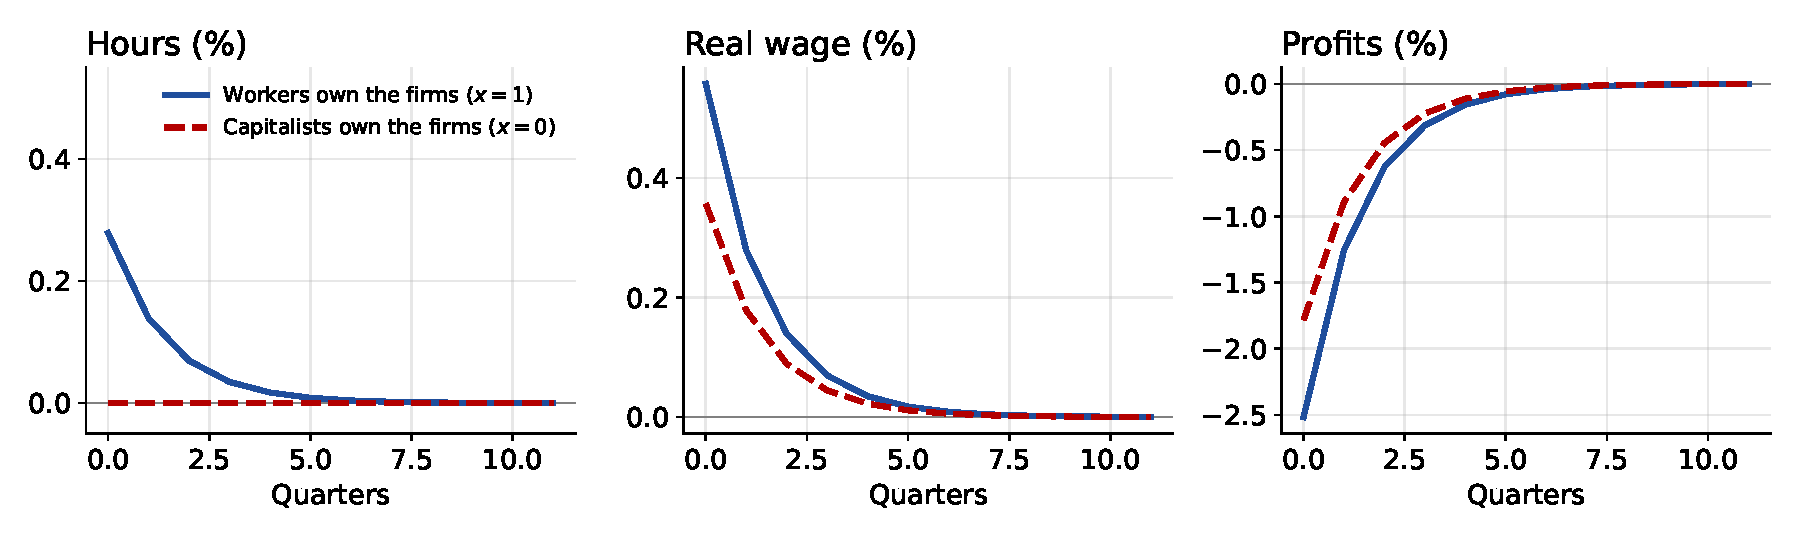
\includegraphics[width=\textwidth]{figs/broer_sticky_prices.pdf}
\end{center}
\begin{itemize}
\item Cut of 25 basis points, persistence 0.5, Taylor rule with $\phi_{\pi}=1.5$
\item Real wage up and profits down in both cases
\item Hours: +0.28\% with $x=1$, and exactly 0 with $x=0$
\end{itemize}
\end{frame}
%
\begin{frame}{Sticky wages}
\begin{itemize}
\item Households are now off their labor supply curve:
\[
\pi_{t}^{w}=\kappa_{w}\left(\varphi L_{t}^{\nu}-\frac{w_{t}}{c_{t}}\right)+\beta\pi_{t+1}^{w}
\]
\item Hours are set by demand, and the real wage barely moves
\end{itemize}
\begin{center}
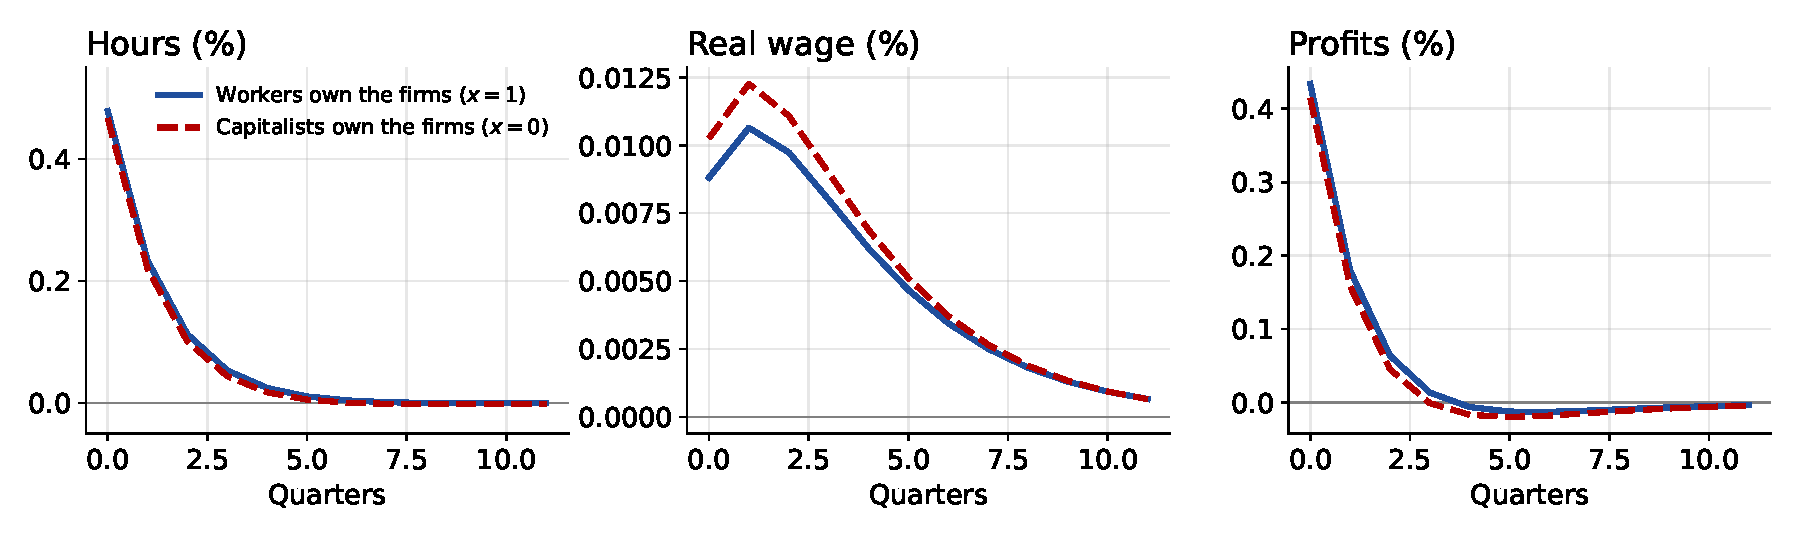
\includegraphics[width=\textwidth]{figs/broer_sticky_wages.pdf}
\end{center}
\begin{itemize}
\item Hours: +0.48\% with $x=1$, and +0.47\% with $x=0$
\item Profits now rise, and who owns the firms hardly matters
\end{itemize}
\end{frame}
%
\begin{frame}{Why we use sticky wages}
With sticky prices only, a rate cut raises output only if
\begin{enumerate}
\item profits fall after a rate cut, while they rise in the data
\item the people who work own the firms, while most workers own little equity
\end{enumerate}
\medskip{}
With sticky wages, output rises through demand, whoever owns the firms
\medskip{}
\begin{center}
\begin{tabular}{lcc}
\hline 
Impact on hours & $x=1$ & $x=0$\tabularnewline
\hline 
Sticky prices & 0.28\% & 0\%\tabularnewline
Sticky wages & 0.48\% & 0.47\%\tabularnewline
\hline 
\end{tabular}
\end{center}
\medskip{}
\begin{itemize}
\item The result is the same in HANK when workers hold the bonds
\item Reference: Broer, Harbo Hansen, Krusell and Öberg (2020, \emph{REStud})
\end{itemize}
\end{frame}

\end{document}
